\documentclass{article}

\usepackage{lmodern}
\usepackage[T1]{fontenc}
\usepackage[utf8]{inputenc}

% Drafting

\usepackage[latexmk]{lwarp}

\usepackage{xcolor,soul}
\usepackage{fullpage}
\usepackage{setspace}
\usepackage{blindtext}
\doublespacing

\definecolor{mwcolor}{HTML}{8af67d}
\definecolor{vgcolor}{HTML}{c88bff} % MPL purple
\definecolor{citecolor}{HTML}{c696f0} % MPL purple


% Tools for leaving todo notes around
\usepackage[colorinlistoftodos]{todonotes}
%% \renewcommand{\todo}{}
%% \renewcommand{\hl}[1]{#1}
\newcommand{\citeme}[1]{%
  \todo[color=citecolor]{%
  \ifstrempty{#1}{[citation needed]}{[cite: #1]}%
  }%
}
\newcommand{\mw}[2]{%
  \sethlcolor{mwcolor}\hl{#2}\sethlcolor{yellow}%
  \ifstrempty{#1}{}{%
    \todo[color=mwcolor]{#1 [MW]}%
  }%                  
}
\newcommand{\vg}[2]{%
  \sethlcolor{vgcolor}\hl{#2}\sethlcolor{yellow}%
  \ifstrempty{#1}{}{%
    \todo[color=vgcolor]{#1 [VG]}%
  }%                  
}


\usepackage{graphicx}
\usepackage[version=4]{mhchem}
\usepackage{siunitx}
\usepackage[hidelinks]{hyperref}
\usepackage{glossaries}
\usepackage[xr,user]{zref} % For cross references to supplemental figures
\usepackage{textgreek}

\newcommand{\nca}[1]{\ce{Li_{#1}Ni_{0.8}Co_{0.15}Al_{0.05}O_2}}
\DeclareRobustCommand{\nmc}[2][]{%
    \ifstrempty{#1}{%
        \ce{Li_{#2}Ni_{y}Mn_{z}Co_{1-y-z}O2}}{}%
    \ifstrequal{#1}{333}{%
        \ce{Li_{#2}Ni_{1/3}Mn_{1/3}Co_{1/3}O2}}{}%
    \ifstrequal{#1}{532}{%
        \ce{Li_{#2}Ni_{0.5}Mn_{0.3}Co_{0.2}O2}}{}%
}

% Techniques
\newacronym{xrd}{PXRD}{powder X-ray diffraction}
\newacronym{uxrd}{µ-XRD}{X-ray microdiffraction}
\newacronym{txm}{TXM}{transmission X-ray microscopy}
\newacronym{xas}{XAS}{X-ray absorbance spectroscopy}
\newacronym{xanes}{XANES}{X-ray absorbance near edge spectroscopy}
\newacronym{iscat}{iSCAT}{optical interferometric scattering microscopy}

% Facilities and organizations
\newacronym{ssrl}{SSRL}{Stanford Synchrotron Radiation Lightsource}

% Chemistry
%\newacronym{ecd}{ECD}{exchange current density}
\newacronym{ecd}{$i_0$}{exchange current density}
\newacronym{od}{OD}{optical depth}
\newacronym{ocv}{OCV}{open circuit voltage}

% Particles in u-XRD mapping
\newacronym{p1}{P1}{particle 1}
\newacronym{p2}{P2}{particle 2}
\newacronym{p3}{P3}{particle 3}


\usepackage{authblk}

\title{Origin of Rapid Delithiation In Secondary Particles Of \nca{} and \nmc{} Cathodes}

\author[1,2,3]{Mark Wolfman}
\author[1]{Brian M.\ May}
\author[4]{Vishwas Goel}
\author[4]{Sicen Du}
\author[5,6]{Young-Sang Yu}
\author[7]{Nicholas V.\ Faenza}
\author[7]{Nathalie Pereira}
\author[8]{Antonin Grenier}
\author[3]{Kamila M.\ Wiaderek}
\author[3]{Ruqing Xu}
\author[9]{Jiajun Wang}
\author[8]{Karena W.\ Chapman}
\author[7]{Glenn G. Amatucci}
\author[4]{Katsuyo Thornton}
\author[1]{Jordi Cabana\thanks{Corresponding author: jcabana@uic.edu}}

\affil[1]{Department of Chemistry, University of Illinois at Chicago}
\affil[2]{Chemical Sciences and Engineering Division, Argonne National Laboratory}
\affil[3]{X-ray Science Division, Advanced Photon Source, Argonne National Laboratory}
\affil[4]{Department of Materials Science and Engineering, University of Michigan}
\affil[5]{Department of Physics, Chungbuk National University}
\affil[6]{Advanced Light Source, Lawrence Berkeley National Laboratory}
\affil[7]{Energy Storage Research Group, Department of Materials Science and Engineering, Rutgers, The State University of New Jersey}
\affil[8]{Department of Chemistry, Stony Brook University}
\affil[9]{Harbin Institute of Technology}

\date{}


\newlength{\figwidth}
\setlength{\figwidth}{3.5in}

\myexternaldocument[si:]{supplement}

\begin{document}

\maketitle

\begin{abstract}
  Most research on the electrochemical dynamics in battery materials
  has focused on the global behavior of the electrode. There has been
  debate within recent literature on the origin of an apparent
  two-phase transformation within layered cathodes for Li-ion
  batteries. The work presented here uses nano-focused X-ray probes to
  measure delithiation \textit{in operando} at the scale of secondary
  particle agglomerates in \nca{} and \nmc{} cathodes during
  charge. After an initial latent phase, individual secondary
  particles undergo rapid, \vg{By stochastic do we mean random
    particles? [MW: yes]}{stochastic}, and largely uniform
  delithiation, which is in contrast with the gradual increase in cell
  potential. These results provide direct evidence that the apparent
  two-phase transition emerges from kinetic limitations experienced by
  a population of secondary particles. Physics-based modeling shows
  that, to reproduce the experimental results, the \gls{ecd} must depend
  on the \gls{xLi}, and that \gls{ecd} should increase rapidly over three
  orders of magnitude when $\gls{xLi} \approx 0.9$. The specifics and
  implications of this jump in \gls{ecd} are crucial to understanding
  the charge-storage reaction of Li-ion battery cathodes.
\end{abstract}

% \listoftodos

\section{[Other papers to consider]}
\begin{itemize}
\item \url{https://pubs.acs.org/doi/pdf/10.1021/acs.nanolett.2c01818}
\item \url{https://onlinelibrary.wiley.com/doi/10.1002/anie.202205394}
\item \url{https://doi.org/10.1021/acs.nanolett.2c01818?urlappend=%3Fref%3DPDF&jav=VoR&rel=cite-as}
\item \url{https://onlinelibrary.wiley.com/doi/10.1002/anie.202205394}
\end{itemize}

%%%%%%%%%%%%%%%%%%%%%%%
\section{Introduction}
%%%%%%%%%%%%%%%%%%%%%%%

% NCA/NMC material
Layered transition metal oxides represent the state-of-the-art
cathode materials for electrochemical energy storage with Li-ion batteries. In order to
meet ever more ambitious performance targets, it is necessary to
improve their efficiency and reliability beyond current
limitations. While layered cathodes provide high theoretical capacity,
only \SI{\approx70}{\percent} is realistically achievable, with a
steeper penalty imposed at higher rates of charge and
discharge\citeme{}. This observation points to kinetic barriers
preventing full utilization of the cathode. Careful observation of
local heterogeneity, combined with detailed simulation of the
underlying electrochemical processes, can reveal details of the
kinetic factors governing these reactions, ultimately leading to
energy storage systems with superior performance.

% TXM/XRD background

Synchrotron X-ray characterization provides several methods to
evaluate heterogeneity within secondary particles of layered cathode
materials\cite{doeff2017}. Among them, \Gls{uxrd} extends the structural characterization
capability of conventional \gls{xrd} with improved spatial
resolution. Incoming X-rays are focused to a sub-micron spot and
scanned over individual secondary particles. At each mapping position,
the diffraction pattern captured by an area detector provides details
of the crystal structure, like the lattice parameters, which can then
be related to chemical states (e.g.\ extent of lithiation). A
complementary technique, \Gls{txm}, produces projection micrographs
showing the optical depth of the object with \SI{\approx30}{nm}
spatial resolution, depending on the instrument configuration. The
tunable nature of synchrotron X-ray sources allows micrographs of the
same field of view to be captured at several energies. To produce
chemical maps, images are collected at a range of energies spanning an
X-ray absorption edge, which produce a separate spectrum for each
pixel in the field of view and a chemical map with chemical
significance (e.g.\ metal oxidation states) after data reduction. For
both techniques, since the individual measurements are projections
through the specimen, the resulting maps show the average state
through the optical axis (perpendicular to the image plane).

The long penetration depth provided by hard X-rays is conducive to
making measurements inside an assembled cell (in-situ) and, ideally,
while the cell is actively cycling (operando). In addition to avoiding
relaxation effects, in-situ measurement allows the same object to be
measured repeatedly at different states of charge. Tracking the same
object during a (dis)charge cycle allows for a direct comparison
between different states of charge and provides a clearer picture of
the evolution of heterogeneity.

%% NCA/NMC background

%% JC: We need to revamp this section. Like Vishwas, I think it gives too
%% much weight to Li2CO3.  I would focus on the fundamentals of the
%% transformation, not aspects that ultimately depend on care and don't
%% even apply to all layered cathodes.

%% jcabana: Ideally, this explanation needs to cover what is known about
%% these fundamentals, so they would cover the Chueh paper and any of the
%% recent papers that we consider relevant.

%% jcabana: The problem of the current intro is that we will be bombarded
%% with papers by the reviewers. The most modern reference is from
%% 2018. This has to do with how long it took to write the paper, but
%% still. this is where we are.

Ensemble \gls{xrd} has shown a mixture of phases in \nca{} electrodes
during the first charge when stored in ambient conditions, unlike the
single-phase (solid solution) transformation seen during subsequent
charge cycles\cite{robert2015}. While a \ce{Li2CO3} surface layer has
been used to explain a seemingly two-phase
transformation\cite{grenier2017}, limitations arising from diffusion
kinetics within the material have also been demonstrated at distinct
Li-site fractions\cite{chapman2020}. Recently, in-situ \gls{xrd} was
used to indirectly study the transformation kinetics of the related
\nmc[333]{} cathode, and showed that interfacial exchange current is a
better explanation than \ce{Li+} diffusion limitations for the
observed pseudo-two-phase behavior\cite{chueh2021}. In the same
report, ex-situ X-ray microscopy revealed secondary particles in
disparate states of charge from one another. While in-situ \gls{xrd}
studies of \nmc[333]{} during first charge generally show a
transformation that is primarily single-phase (solid
solution)\cite{hulzen2018,ahn2017,zhou2016-2}, some studies reveal two
crystallographic phases with a small difference in \emph{a} and
\emph{c} lattice parameters coexisting over a narrow range of
delithiation compared to \nca{}\cite{yoon2006,hua2018}. The oxidation
dynamics of these layered cathode materials warrant further study to
clarify the nature of the chemical transformation, especially in view
of locating the onset and progression of heterogeneity, within and
among the secondary particles that typically compose a cathode.


The work described here further examined the heterogeneities present
in secondary particles of established layered cathode materials,
namely \nca{}, \nmc[333]{}, and \nmc[532]{}. A combination of operando
\gls{uxrd} and \gls{txm} \gls{xas} experiments probed the
inter-particle heterogeneity. While the cell potential and prior
reports of ensemble \gls{xas} indicated a smooth transition to higher
oxidation state upon delithiation\cite{deb2005,muto2009}, individual
particles exhibited a sharp and stochastic transition from an initial,
latent state to one containing highly oxidized \ce{Ni}. We refer to
this phenomenon rapid or accelerated delithiation. Physics-based
simulations were then conducted to determine the role of fundamental
electrochemical processes in generating this rapid delithiation
behavior, which showed that this behavior due to a significant
increase in \gls{ecd} covering several orders of magnitude during
delithiation. These observations highlight the decoupling between
single-particle dynamics and the macroscopic response in battery
electrodes even when they follow mechanisms of solid solution. The
identification of \gls{ecd} as controlling parameter in these
materials redirects models away from a focus on mass diffusion.

%%%%%%%%%%%%%%%%%%%%%%%%%%%%%%%%%%%%%%%%%%%%%%%%%
\section{Operando observations of single particle dynamics}
%%%%%%%%%%%%%%%%%%%%%%%%%%%%%%%%%%%%%%%%%%%%%%%%%

%% \subsection{\Gls{uxrd} - Interparticle Dynamics}

Secondary particles of \nca{} were tracked during their first charge
and discharge using operando \gls{uxrd} mapping (Figure \ref{fig:uxrd}). Dilute
(\SI{20}{\percent} w/w) \nca{} electrodes were used to isolate the
response of individual particles from each other. The introduction of large amounts of carbon black to dilute the particles had the beneficial effect of ensuring that the electronic conductivity of the electrode was not limiting, but it contributed to the faradaic processes on charge due to irreversible interactions with the electrolyte\cite{kostecki2014}, artificially extending the charging process (Figure \ref{fig:uxrd}c). For each X--Y
mapping position, the individual 2D diffraction signals were
integrated to one-dimensional patterns and converted from angular
domain ($2\theta$) to the \gls{q} domain, which, in turn, relates to the \gls{d} spacing between planes in the crystal lattice through
$d=\frac{2\pi}{\vert\vec{q}\vert}$. While data were collected
with \SI{\approx500}{\nano\meter} spatial resolution, smaller than the
particle agglomerates, all patterns from the same particle agglomerate
at a given time stamp during the reaction were summed for the analyses
presented here (Figures \ref{fig:uxrd}a,b and
\zref{si:fig:xrd-echem}), to focus the analysis on the particle, rather than domain, dynamics. In all cases, the pristine state matched the
literature results for \nca{} \cite{novak2015}, with the exception of
an extra feature at $\gls{q}\approx\SI{3.6}{\per\angstrom}$ due to
metallic \ce{Li} (PDF \#00-001-1131). Small extraneous peaks occurred
due to random aberrations in individual pixels on the diffraction
detector (Figure \zref{si:fig:xrd-echem}).

During (de)lithiation, the diffraction peaks for \gls{p1} began to shift in \gls{q} soon after the onset of oxidation (Figure \ref{fig:uxrd}a), following the
same overall trajectory as reported for the ensemble
average\cite{robert2015}. This similarity and the absence of peak
splitting indicates that individual particles followed a single
phase mechanism, with no fictitious phase separation induced by
surface impurities \cite{grenier2017}. The most characteristic changes
can be observed at the (003) and (104) reflections. The former showed
an initial decrease in \gls{q} (higher \gls{d}) (Figure
\ref{fig:uxrd}a), followed by a sudden increase in \gls{q} beyond the
initial state, representing an expansion then contraction along the
$c$ axis during delithiation\citeme{}. The (104) diffraction peak
gradually shifted to higher \gls{q} (lower \gls{d}) upon removal of
\ce{Li} (Figure \ref{fig:uxrd}b), reflecting the balance between the
trend along $c$, which is pseudo-parabolic, and the continuous decrease in the $a$
dimension.\cite{robert2015} While the peak positions of \gls{p2}
(Figure \zref{si:fig:xrd-echem}b) underwent similar changes, the peaks
did not begin shifting until the electrochemical cell had reached a
higher potential \SI{\approx4.5}{\volt}. During discharge, peaks in
both \gls{p1} and \gls{p2} shifted to lower \gls{q} at approximately
the same rate.

The evolution of the lattice parameters for each particle as a
function of cell potential were extracted from refinements of the
diffraction patterns (Figures \ref{fig:uxrd}d and
\zref{si:fig:cell-pars}). Both particles exhibited lattice parameters
at the end of charge and discharge consistent with full delithiation
and relithiation, respectively\cite{novak2015}. The trends followed by
the lattice parameters during the reaction again agreed with
measurements of the ensemble average in the
literature\cite{novak2015, faenza2018}, but their timing with respect to the experiment differed. The lattice parameters for
\gls{p1} and \gls{p2} began shifting at cell potentials below
\SIrange{3.0}{3.8}{\volt} and at \SI{\approx4.5}{\volt}, respectively
(Figure \ref{fig:uxrd}d). All in all, the rates of delithiation of
each individual particle were different from the electrochemical
response collected for the whole electrode. Both \gls{p1} and \gls{p2}
achieved the same level of delithiation at the end of the charge
sequence, observed in Figure \ref{fig:uxrd}e and by the peak positions
in Figures \ref{fig:uxrd}a,b and \zref{si:fig:ind-peaks}. Since
\gls{p2} did not start delithiating until late in the charge sequence,
its maximum rate of delithiation was more than double that of
\gls{p1}. This observation is unexpected for solid solutions, since there is no thermodynamic activation barrier toward nucleation of segregated phases.

\vg{I think we should provide a
  brief explanation in the difference between the phase-transformation
  led heterogeneity (like in LFP) vs.\ the heterogeneity observed here
  in the introduction.}{}

%% \subsection{u-XRD - Rates of (De)lithiation}
\newpage % temporary to keep comments from overrunning
Further insight into rates of delithiation of each particle during the reaction was
extracted from the relationship between \gls{xLi} in \nca{x} and
lattice parameters collected with PXRD in the literature.\cite{robert2015} (Figure
\zref{si:fig:xrd-echem}), and plotting the value against the time elapsed in the experiment. Figure \ref{fig:uxrd}e shows the \ce{Li}
content obtained from the \emph{c} lattice parameter at selected time stamps for each of the
two \nca{x} particles during the first charge-discharge cycle. Similar trends
were observed when calculating \ce{Li} content using the \emph{a}
parameter (Figure \zref{si:fig:rates}). In these plots, to allow for
an easier comparison between experiments and simulation, the Li
content was plotted against the ratio of time passed since current was
applied to the total time to reach the charge cutoff potential ($t_c$), given the decoupling between the macroscopic rate of the experiment and that of individual particles.

For both \gls{p1} and \gls{p2}, the rate of delithiation, estimated
from the slope in Figure \ref{fig:uxrd}e, was initially low,
proceeding at \SI{\approx0.025}{\ce{Li}\per\hour}, or C/40. Once the
overall content of the particle reached \Li{0.9}, the reaction
dramatically accelerated nearly 10-fold, to
\SI{\approx0.3}{\ce{Li}\per\hour}, or C/3, until an average
composition \Li{0.5}, followed by renewed deceleration, to
\SI{0.1}{\ce{Li}\per\hour}, or C/10, leading to a rather small change
in Li fraction until the sign of the current was reversed. In the case
of \gls{p2} there was very little delithiation for the first
\SI{0.8}{t_c}. However, once it began rapid delithiation, the Li
fraction evoled in a similar manner as \gls{p1}, with a 20-fold
acceleration at \Li{0.9} to \SI{\approx0.66}{\ce{Li}\per\hour}, or
C/1.5, which lasted until an average particle composition \Li{0.5},
after which the rate fell below \SI{0.1}{\ce{Li}\per\hour}, or C/10,
for the remainder of the delithiation process. The divergence in charging rates during a galvanostatic experiment has been recently reported by others using optical microscopy. However, our ability to relate specific signatures with Li content using its well-established dependence on \gls{d} allow us not only to pinpoint that the rate acceleration happens at specific points of the reaction (between \Li{0.9} and ~\Li{0.6}), but also estimate the actual rate of the process at each stage.

The discharge of the cell proceeded more quickly than charge, with the consequence that less data points were captured for quantification. Nonetheless, the process returned the cell parameters of both particles to values close to the pristine state, indicating degrees of reversibility comparable to the literature.\cite{robert2015} The change in cell parameters was smoother than upon charge, with no obvious evidence of acceleration. It is worth noting that, while the end values were similar, the trajectory of both a and c parameters was not quantitatively the same. For instance, the c parameter peaked at 14,48 and 14.35 A on charge and discharge, respectively. This evolution suggests that full delithiation introduces irreversible structural changes that affect the dependence of cell parameters on Li content. To the best of our knowledge, this issue has not been explored in the literature and demands dedicated operando PXRD experiments. Upon discharge of the
cell, i.e.\ after \SI{1.0}{t_c}, both particles relithiated quickly at
the initial stages, with the consequence that too few data points were
captured for a reliable quantification. When the lattice parameters
reached values corresponding to \Li{0.8}, the rates fell to
\SI{\approx0.025}{\ce{Li}\per\hour}, or C/40. \kt{Just to make sure,
  you are saying the discharge process is similar to the charge
  process?  I think it's best to provide more details since I don't
  usually think of the discharge process to be comparable to charge
  process (it's opposite).  I had to read this paragraph many times to
  try to understand it, and I think it could be clearer. (MW:
  Brian?)}{The behavior was qualitatively comparable to the first
  charge, including} \gls{p1} delithiating earlier than \gls{p2}.


%% \subsection{TXM - \nmc{}}

%% \subsubsection{\nmc[333]{} Inter-particle Dynamics}

A second set of independent experiments was pursued to evaluate the
reproducibility of the varying delithiation rates observed among
particles by the operando \gls{uxrd} mapping. In particular, we
employed operando \Gls{txm} \gls{xas} of \nca{} secondary particles
during charging to probe \ce{Ni} oxidation states at high spatial
resolution. Framesets containing multiple particles were collected
during the first galvanostatic charge (Figure
\ref{fig:txm-nca}a). Localized \gls{xas} K-edge spectra were averaged
over all pixels in a single secondary particle. XAS measurements of the ensemble average of electrodes showed that, upon delithiation, there was a
progressive increase in the energy of the absorption edge and
the associated energy of maximum absorbance, or whiteline (Figures
\zref{si:fig:isobestic-point} and \zref{si:fig:kedges}), consistent with literature observations of \ce{Ni^{2+}} oxidation to \ce{Ni^{4+}}.\cite{deb2005}\cite{muto2009} Therefore, the whiteline energy was used as a proxy for
\ce{Ni} oxidation, which is the dominant redox process in \nca{} and
\nmc{}. Figure \ref{fig:txm-nca}c shows the changes in
ensemble-average \ce{Ni} K-edge \gls{xas} spectra for \nca{} across
known states of delithiation; these spectra were used as calibration
data for the in-situ experiments. The resulting plots of average
state-of-charge for each particle as a function of time are shown in
Figure \ref{fig:txm-nca}d.

Initially, the mean whiteline energies of the particles studied did
not change, indicating no \ce{Ni} oxidation. Between
\SIrange{0.4}{0.6}{t_c}, the whiteline energies increased rapidly for
all particles, reaching \SIrange{75}{100}{\percent} \kt{When working
  with cathode and lithium site fraction, I prefer using depth of
  discharge instead so that 0 and 1 do not need to be flipped.  Or
  just stick with lithium site fraction rather than going back and
  forth.  SOC and DOD sounds more like it's about cell, so it might be
  better to stick with site fraction. [MW: I agree, we need to find
    out from YS how he defines 100\% SOC in order to translate to Li
    fraction]}{state-of-charge}. Although several particles oxidized
concurrently, there was no clear preference for when particles
  began rapid oxidation. The analysis produced instances where the trend in whiteline appeared to shift toward lower energy upon
reaching their maximum state-of-charge, suggesting \ce{Ni} reduction may have occurred, presumably due to the instability of
\ce{Ni} in high oxidation states\citeme{}, resulting in oxygen
loss. Overall, the observation of rapid particle oxidation despite the constant current applied to the cell was in
agreement with \gls{uxrd} above
(Figure \ref{fig:uxrd}).

\begin{table}
  \begin{tabular}{c c c | c c c}
    \multicolumn{3}{c|}{\nmc[333]{x}} & \multicolumn{3}{c}{\nca{x}} \\
    x & Whiteline /eV & \textDelta{} /eV & x & Whiteline /eV & \textDelta{} /eV \\
    \hline\hline
    0.945 & 8353.98 & 0.21 & 1.00 & 8348.84 & 0.00 \\
    0.751 & 8354.72 & 0.94 & 0.80 & 8349.61 & 0.78 \\
    0.570 & 8355.45 & 1.68 & 0.60 & 8350.14 & 1.30 \\
    0.386 & 8356.12 & 2.35 & 0.25 & 8350.78 & 1.95 \\
    0.257 & 8356.43 & 2.66 & 0.00 & 8351.16 & 2.32 \\
  \end{tabular}
  \caption{Reported energies of \ce{Ni} K-edge whiteline. In-situ
    \gls{xas} of \nmc[333]{x} (Ref.\ \cite{deb2005}) and ex-situ
    \gls{xas} \nca{x} (Ref.\ \cite{muto2009}). Data extracted from
    published figures using
    WebPlotDigitizer\cite{webplotdigitizer}. Relative shifts in
    whiteline energy (\textDelta{}) calculated as difference from
    fully lithiated state ($x=1$).}
  \label{tab:bulk-xas-extraction}
\end{table}

\newpage % temporary to keep comments from overrunning
%%%%%%%%%%%%%%%%%%%%%%%%%%%%%%%%%%%%%%%%%%%%%%%%%
\section{Relevance to other cathode materials}
%%%%%%%%%%%%%%%%%%%%%%%%%%%%%%%%%%%%%%%%%%%%%%%%%

%% \subsubsection{\nmc[532]{}}

To evaluate the similarity between the oxidation behavior of \nca{}
and other layered cathode compositions, similar \gls{txm} \gls{xas}
experiments were performed on cells containing dilute \nmc[333]{} and
\nmc[532]{} layered cathodes (Figure \ref{fig:txm-nmc}). We note that
\nmc{} particles (Figure \ref{fig:txm-nmc}a) were less spherical in
shape as compared to \nca{} (Figure \ref{fig:txm-nca}a). The mean
optical depth for all foreground pixels in the frame was used for
evaluating overall oxidation (Figures \ref{fig:txm-nmc}b,c). As
expected, \nmc[333]{} exhibited a lower initial whiteline energy than
\nca{}\cite{deb2005,muto2009}, matching the contrast between \ce{Ni^{2+}} and \ce{Ni^{3+}}. Similar to \nca{}, spectra for both
\nmc{} cathodes showed an increase in the whiteline energy, which is
in agreement with the literature\citeme{}. To estimate the state of
charge, the evolution of the whiteline was compared to the lowest
value observed for any particle in the field of view during the
operando experiment, reported here as \textDelta{}whiteline. A
parametric function was fit to each pixel's full spectrum, and the
whiteline energies were extracted from the fit parameters. \kt{If so,
  why was it not applied in the previous case?  You probably want to
  offer some explanation. [MW: Real answer: because two different
    people did the analyses. You bring up a good point, though. Any
    thoughts on how to answer this?]}{This approach provided higher
  precision and was more tolerant of noise between frames, allowing
  for faster time resolution.} For both \nmc{} materials, the same
initial latent phase and subsequent rapid oxidation were seen (Figures
\ref{fig:txm-nmc}d,e). The initial rapid \ce{Ni} oxidation resulted in
changes in whiteline energy for \nmc[333]{} of
\SI{\approx3}{\electronvolt} and \nmc[532]{} of
\SI{\approx2.5}{\electronvolt}, reflecting the lower starting
concentration of \ce{Ni^{2+}} in \nmc[333]{}. The experiment using
\nmc[532]{} did not reach the same overall state of charge as those
using \nmc[333]{} and \nca{} due to loss of X-rays. For \nmc[333]{},
once rapid oxidation had occurred, a subsequent gradual increase to
\SI{4.1}{eV} was observed, consistent with the final phase of slower delithiation observed for NCA using \gls{uxrd}. The total change in whiteline energy for
all observed secondary particles was \SI{>4}{eV} (Figure
\ref{fig:txm-nmc}d). While ensemble \gls{xas}
studies\cite{deb2005,muto2009} did not reach the \SI{4.7}{V} cell
cut-off potential needed for full lithium extraction (hence full
\ce{Ni} oxidation), extrapolation of the trend in Table
\ref{tab:bulk-xas-extraction} and Figure
\zref{si:fig:bulk-xas-extraction}a predicts a change in whiteline
energy upon full delithiation of \SI{\approx3}{eV}. This discrepancy
between particle-level and ensemble average \ce{Ni} oxidation suggests
that an appreciable portion of the particles in the specimens measured
by ensemble \gls{xas} had not reached their fully oxidized states.

In summary, all layered cathode chemistries studied here exhibited
individual secondary particles undergoing rapid delithiation at
various times during galvanostatic delithiation. This behavior was
observed experimentally by two independent mapping techniques
(\gls{uxrd} and \gls{txm}), with very different energies of the X-ray beam
(\SI{\approx8}{\kilo\electronvolt} for TXM vs
\SI{25}{\kilo\electronvolt} for \gls{uxrd}). The persistence of the
phenomena suggests that the behavior is inherent
to layered cathode materials rather than being an artifact of the
techniques, and is consistent with previous reports using other
techniques on related \nmc{} and \ce{LiCoO2} layered
materials\cite{chueh2021,rao2021,wang2020-6}.


\section{Simulation of single particle dynamics}

%% Electrochemical dynamics simulations to identify the origin of the
%% accelerated delithiation

Our \gls{uxrd} experiments clearly show that changes in rate of delithiation
occur at similar Li contents in the particles, suggesting that the fundamental electrochemical properties
are strongly dependent on the state of charge. While the observed
phenomenon of accelerated delithiation is reminiscent of the
interparticle phase separation predicted in lithium iron phosphate
\citeme{VG/KT?}, it does not apply here because the system under
investigation is not a two-phase system in thermodynamic
equilibrium. To gain further insight into the observed accelerated
delithiation, we performed physics-based particle-level simulations of
\nca{x}. While the computational expense (resulting from large changes
in properties with varying x) does not allow a parametric study of
many-particle simulations, it was sufficient to consider 8 particles
with diameters ranging from \SIrange{4}{11}{\micro\meter} in the
cathode and a thin Li metal layer as the anode to survey the parameter
space and support the finding with one larger (30-particle)
simulation. More details on the model geometry, equations, and
parameters are provided in the \ref{sec:methods} Section and the
Supporting Information.

%% The delithiation process of the cathode particles involves (a)
%% transport of Li ions in the electrolyte, (b) transport of Li in the
%% active material particles, (c) electrochemical reaction at the active
%% material surface, and (d) transport of electrons in the cathode. Due
%% to the large volume fractions of the pore phase and the carbon
%% additive in the cathode, we can ignore the effects of mechanisms (a)
%% and (d).
The effect of the electrochemical reaction that occurs at the
interface between the active material and the electrolyte phase can be
studied using the \gls{ecd}. Similarly, the effect of the transport of
\ce{Li+} can be studied using the \gls{D_s}. Both of these quantities
are dependent on the \gls{xLi} in the particles. Therefore, we
performed sensitivity analyses with respect to various functional
forms and values of \gls{ecd} and \gls{D_s}, including the ones
reported in literature\citeme{VG/KT?} and constructed for this work to qualitatively
reproduce rapid delithiation. The details of these forms are provided
in the Supporting Information. %% Our sensitivity analyses generated
two
%% major insights: first, rapid delithiation is a reaction-controlled
%% phenomenon; second, this phenomenon is strongly observed only when
%% $i_0$ changes more than two orders of magnitude during charging
%% . Furthermore, a similar change in $D_s$ does not exhibit rapid
%% delithiation without a large change in $i_0$. In the following, we
%% discuss these insights in a greater detail.

Figure \ref{fig:model-1}b shows the evolution of volume-averaged
Li-site fraction, $\left\langle \gls{xLi} \right\rangle$, of the 8
particles for \SI{0.05}{\ampere\per\ampere\hour} (C/20) charging
obtained using a model form of \gls{ecd} that was constructed based on
the recent studies of \nca{} \cite{chueh2021} and NMC \cite{tsai2018,
  mukherjee2017, chiang2020}. Figure \ref{fig:model-1}a shows the
dependence of the model form of \gls{ecd} on \gls{xLi} that exhibited
rapid delithiation similar to the experiment. The model \gls{ecd} is a
smoothed step function with a significant increase in the value with
decreasing x around a transition point ($\gls{xLi}\approx0.9$). As can
be seen in Figure \ref{fig:model-1}b, all the particles exhibit rapid
delithiation. When a particle reaches $\left\langle \gls{xLi}
\right\rangle\approx0.9$, \gls{ecd} begins to increase rapidly and
thereby causes the particle to experience an accelerated reaction rate
as it is further delithiated. This acceleration causes the particle to
contribute the majority of the applied current, which stagnates the
delithiation rate of other particles that have not reached the
transition point under galvanostatic conditions. By the time the
particle completes its accelerated delithiation, another particle
undergoes this transition and thus rapid delithiation. This cycle
repeats until the last particle undergoes rapid delithiation.  We note
that no rapid delithiation was observed when the traditional form of
\gls{ecd} ($\propto\sqrt{gls{xLi}(1-\gls{xLi})}$ \cite{newman1993,
  newman1994, newman1995, newman1996}) is used, as shown in Figure
\zref{si:fig:x-evolution}.

The oscillations observed in $\left\langle \gls{xLi} \right\rangle$ in
Figure \ref{fig:model-1}b arise due to the large difference between
minimum and maximum values of \gls{ecd} used in these
simulations. This large difference can cause a particle undergoing the
aforementioned transition to deliver more than the applied current,
which induces already delithiated particles to lithiate slightly. Such
phenomena under a galvanostatic condition have also been observed in
\ce{Li_{x}FePO_{4}}, for which the acceleration occurs due to the
thermodynamics of the phase-separating material
\cite{thornton2015}\citeme{KT: Vishwas, I will provide them; please
  add.}. The ensure that the results from the 8-particle simulations
are not artificially affected by the small number of particles
simulated, we performed a simulation with 30 particles; the details of
the simulation are provided in the Supporting Information. The results
are provided in Figure \ref{fig:model-1}c. First, rapid delithiation
is observed for all of the particles even in a larger system, which
shows that such behavior is likely intrinsic to the material. Second,
the amplitudes of the oscillations decrease in the simulation with 30
particles as compared to the 8-particle system, which suggests that
oscillations may not occur in very large systems such as practical
electrodes.  Confirming whether or not such oscillations occur in a
physical system would require higher chemical and temporal resolutions
than what is possible with today's experimental techniques.

Next, we studied the effect of a model \gls{D_s} form that has the
same form as the model \gls{ecd} above, as shown in Figure
\ref{fig:model-2}a. Note that the traditional form of \gls{ecd} was
used for this simulation and initial $\left\langle \gls{xLi}
\right\rangle$ is set to \num{0.95} instead of \num{0.99} in this
simulation to avoid unphysical situations such as $\left\langle
\gls{xLi} \right\rangle > 1$, which can arise from a numerical error
caused by a rapid change in \gls{D_s} with respect to
\gls{xLi}. Figure \ref{fig:model-2}b shows the evolution of
$\left\langle \gls{xLi} \right\rangle$ during charging of the
8-particle system at \SI{0.05}{\ampere\per\ampere\hour} (C/20) with
the model \gls{D_s}. Although accelerated delithiation is observed for
smaller particles, its extent is much smaller than that observed
above. For a particle to exhibit rapid delithiation, the flux at the
particle-electrolyte interface needs to increase rapidly in a short
duration of time. Such an increase in the flux cannot be realized even
if the diffusion function has a step-function-like dependence on
\gls{xLi} because the diffusivity (hence, diffusion flux) only
increases in the shell of the particle close to the particle surface;
the particle bulk continues to have lower diffusivity. In other
words, the entire particle does not undergo rapid delithiation;
instead, only the shell close to the particle surface exhibits such
behavior. Furthermore, the experimental measurements show that the
Li-site fractions within the particles are spatially uniform during
charging (\kt{Which figure [VG: Maybe S15]}{Figure} \todo{Sxx}), which
suggests that Li diffusion is not the limiting mechanism in the
experiment. Indeed, the simulation result also shows \todo{XXXX} for
the values of \gls{D_s} obtained from the literature, as well as the
step form of \gls{D_s} having \todo{XXX} smaller value (\vg{I will
  make this edit post the revision from Mark and Jordi. }{or something
  like this -- Vishwas, please edit}). Hence we can rule out a strong
dependence of \gls{D_s} on \gls{xLi} as the underlying cause of rapid
delithiation.

Based on the insights generated above, we conclude that rapid
delithiation in \nca{} particles is controlled by the surface reaction
kinetics, rather than the bulk \ce{Li+} diffusion dynamics in the
active material. Furthermore, \kt{Can we say that the rate of the
  rapid delithiation is unaltered?  If it's [VG: I need to see if I
    have the data from Sicen for this.]}{the rapid delithiation
  observed} in the 8-particle model is also observed in a larger
system with 30 particles, which demonstrates that it is not an
artifact of the small number of particles simulated. The results from
our deterministic modeling study agrees well with the stochastic
simulations performed by Park et al.\cite{chueh2021}, where the
authors showed that the accelerated delithiation (termed
electro-autocatalysis by the authors) is controlled by the surface
reaction and not the solid-state diffusion. Furthermore, the authors
reported a rapid increase in \gls{ecd} at the \nca{} particle surface
as the delithiation progresses, albeit with an exponential dependence.


%%%%%%%%%%%%%%%%%%%%%
\section{Conclusion}
%%%%%%%%%%%%%%%%%%%%%

Operando X-ray characterization of layered cathodes in assembled
Li-ion cells showed rapid and stochastic oxidation within the cathode
at the level of secondary particle agglomerates. This behavior was
consistent across cathodes with several transition metal compositions,
and when measured by
two distinct X-ray characterization modalities. The robustness with
which this effect was measured demonstrates it to be inherent to
layered cathode materials. Subsequent modeling of the electrochemical
dynamics showed the origins of this rapid delithiation to be the
result of a dramatic increase in the \gls{ecd}. It was found that a
change of three orders of magnitude in \gls{ecd} at $\gls{xLi}\approx
0.9$ to reproduce the experimental results. Rapid stochastic
delithiation explains the apparent two-phase behavior reported by
conventional \gls{xrd}: it is an emergent property resulting from the
ensemble-average nature of the technique rather than being inherent to
the thermodynamics of layered cathodes. The
spectromicroscopy results presented here reveal that individual particles can reach a higher state of charge than
the global average during cycling, highlighting the heterogeneity within the
electrode and the need for experimental techniques such as those
applied here that provide spatial, temporal and chemical resolutions.

\kt{Do we know that this is generically true?  The work examined two
  systems and there are many?  Some may be two phase systems.}{These
  results show that the electrochemical reaction during discharge of
  layered cathodes is kinetically limited by reactions at the surface
  of the secondary particles.} \kt{?? I don't think this was
  discussed?  If so, maybe it was too brief.  Please expand it within
  the text (before the summary).}{At a given Li composition, the
  difference between the equilibrium reduction potential and the
  applied potential represents a thermodynamic irreversibility in the
  system, and thus a reduction in the energy storage efficiency
  relative to the theoretical limit.} \kt{I don't think this was
  discussed or demonstrated — theoretically, this just means that it
  will be utilized at a later time.}{Furthermore, the observation that
  some particles remain lithiated relative for the ensemble average
  equates to a reduction in the usable capacity of the battery.} These factors present areas of improvement for the performance of
layered cathode materials, which could be realized with further
research into the origin of the significant increase in \gls{ecd}
during charging.

%%%%%%%%%%%%%%%%%%%%%%%%%%%%%%%%
\section*{Materials and Methods}
\label{sec:methods}
%%%%%%%%%%%%%%%%%%%%%%%%%%%%%%%%

\subsection*{\gls{uxrd} Mapping}

The \nca{} composite electrode tape was cast in a dry room (dew point
of \SI{<-35}{\celsius}) using the Bellcore method \cite{warren1996}. A
mixture of \nca{}, poly(vinylidene fluoride-co-hexafluoropropylene)
(PVDF-HFP, Kynar 2801, Elf Atochem), carbon black (Super P, MMM),
propylene carbonate (Aldrich), and acetone (Aldrich) was used for the
casting slurry. After casting, the tape was allowed to dry in air, and
then the propylene carbonate plasticizer was extracted by soaking the
tape in 99.8\% anhydrous diethyl ether (Aldrich). The electrode tape
had a mass composition of \SI{20}{\percent} active material,
\SI{20}{\percent} carbon additive, and \SI{60}{\percent} binder. Prior
to storage in the Ar-filled glovebox, the tape was dried under vacuum
at \SI{120}{\celsius} overnight.

The AMPIX electrochemical cell was utilized to allow X-ray penetration
through the electrode \cite{borkiewicz2012}. Lithium metal was used as
the counter electrode and the electrolyte was composed of 1M
\ce{LiPF6} in a 1:1 mixture of ethylene carbonate:dimethyl
carbonate. Glass fiber served as the separator.

Diffraction maps were collected at the microprobe beamline at sector
34 at the Advanced Photon Source (APS), Argonne National Laboratory
(ANL). An incoming monochromatic beam at \SI{25}{\kilo\electronvolt}
(\SI{0.4959}{\angstrom}) with a size of approximately \num{0.5} x
\SI{0.5}{\micro\meter} was shone through the AMPIX cell onto the
sample. The intensity of the diffracted beam was collected in
transmission geometry by a MAR165 CCD detector, with 4096 x 4096
pixels, each measuring \SI{40}{\square\micro\meter}, used in 2 x 2
binning mode.

Particle locations were determined through absorption contrast imaging
over the \ce{Ni K_\alpha} emission line at
\SI{\approx8}{\kilo\electronvolt}. Once particles were located, the
sample was moved relative to the beam using a step size of
\SI{1}{\micro\meter} and an exposure time of
\SI{10}{\second}. Two-dimensional diffraction maps were collected in
this manner continuously over the charge-discharge cycle. At each
exposure, or mapping position, a single full 2D diffraction pattern,
averaging over the depth of the material, was collected (an example is
seen in \zref{si:fig:2Ddiffraction}). After one map was collected for each
particle, a positive current was applied so that the charge rate would
be c/20 (in which removal of a full \ce{Li} equivalent would complete
in \SI{20}{\hour}). The cut-off potential for the cell was set for
\SI{4.8}{\volt}, to ensure a complete oxidation of the \nca{}. After
holding the cell near \SI{4.8}{\volt} for several hours, the cell was
discharged at a negative current equal in magnitude to that of the
charge. The data was collected using EPICS channel-access data
acquisition and control software.

The 2D diffraction data collected by the beamline was integrated using
the FIT2D software package developed by
ESRF\cite{hausermann1996,hammersley1997}. The integrated data was
processed with the Scimap analysis package\cite{scimap}, in which the
determination of the peak position yielded a set of unit cell
parameters for each mapping position, which were plotted using
Python. An ensemble diffraction pattern for each particle at each
state of charge was obtained by summing the patterns at each mapping
position. These patterns underwent batch Le Bail refinement by the
TOPAS software developed by Bruker to produce plots of unit cell as a
function of charge-discharge for each particle as a whole.

\subsection*{\textit{Ex-situ} X-ray absorption spectroscopy - \nca{}}
To obtain standard spectra of \nca{} (NAT-1050) with respect to the
states-of-charge, dense composite electrodes were fabricated by mixing
the pristine \nca{} with acetylene black and polyvinylidene difluoride
(PVDF) in 80:10:10 ratio in N-methylpyrrolidone. The resulting slurry
was cast onto a pre-weighed Al foil disk, dried at room temperature,
followed by a heat treatment of \SI{120}{\celsius} under vacuum for
\SI{12}{\hour}. The composite electrodes were assembled in 2032 coin
cells using lithium foil as both counter and pseudo-reference
electrode, and Celgard 2400 separator soaked in a 45:55 mixture of
ethylenecarbonate and dmiethyl carbonate containing \SI{1}{\molar}
\ce{LiPF6} as electrolyte. All cell assembly and sample manipulation
was performed in an Ar-filled glovebox. Galvanostatic cycling at a
\SI{0.05}{\ampere\per\ampere\per\hour} (C/20) rate (defined as the
current density for full delithiation of \nca{} in \SI{20}{\hour}) was
performed between \SIrange{3.0}{4.8}{\volt} vs.\ \ce{Li+/Li^0} using a
Bio-Logic VSP potentiostat/galvanostat. The reference powders for
\nca{} were harvested from Li metal half cells charged to specific
state-of-charges (\SI{25}{\percent}, \SI{50}{\percent},
\SI{75}{\percent}, and \SI{100}{\percent}) and heat-sealed in
polyethylene to minimize \ce{O2} and \ce{H2O} exposure. Ni K-edge
\gls{xas} transmission spectra were collected for the discrete states
of charge and the pristine state by at beamline 4-1 at the \gls{ssrl},
in transmission mode using a Si (220) double crystal monochromator
(Figures \ref{fig:txm-nca}c). A Ni metal standard foil located in
front of a reference ion-chamber was measured simultaneously with each
spectral sample for energy calibration. All data processing, including
normalization of transmission spectra was carried out using the
software {SIXPACKS} \cite{lai2011}. Pre-edge background subtraction
and \gls{xanes} normalization were carried out by fitting a linear
polynomial to the pre-edge region and a quadratic polynomial to the
post-edge region of the absorption spectrum. All \gls{xanes} spectra
were linearly calibrated using the energy threshold $E_0$ of the
reference Ni foil determined from the first derivative peak of the
spectrum.


\subsection*{TXM - \nca{}}

To visualize the macroscopic electrochemical properties of
single-isolated \nca{} (NAT-1050) secondary powders, diluted and
thinner composite electrodes were fabricated by mixing the pristine
\nca{} with acetylene black and polyvinylidene difluoride (PVDF) in
20:50:30 ratio in N-methylpyrrolidone. The resulting slurry was cast
onto a pre-weighed Al foil disk with a thickness of
\SI{30}{\micro\meter}, dried at room temperature, followed by a heat
treatment at \SI{120}{\celsius} under vacuum for \SI{12}{\hour}. The
composite electrodes were assembled in \mw{modified how?
  YSY?}{modified} 2032 coin cells using lithium foil as both counter
and pseudo-reference electrode, and Celgard 2400 separator soaked in a
45:55 mixture of ethylenecarbonate and dmiethyl carbonate containing 1
M \ce{LiPF6} as electrolyte. To ensure sufficient transparence to the
X-ray beam, holes were punched in the cell cases. After cell assembly,
the holes in the cell cases were sealed with \SI{1}{\micro\meter}
thick \ce{Si3N4} windows (Norcada NX5200F) using Torr-Seal
vacuum-rated epoxy. All cell assembly and sample manipulation was
performed in an Ar-filled glovebox. Operando \gls{txm} was performed
at the 54 pole wiggler beamline (BL 6-2) at the \gls{ssrl}
\cite{yun2008}. Galvanostatic cycling at a
\SI{0.05}{\ampere\per\ampere\per\hour} (C/20) rate was performed
between \SIrange{3.0}{5.0}{\volt} vs.\ \ce{Li+/Li_0} using a Bio-Logic
VMP potentiostat/galvanostat. The absorption contrast images
(\SI{0.5}{\second} exposure time, \ysy{get value}{XX} repetitions,
binning 2, $\rm 1024\times 1024$ pixels) were captured across Ni
K-edge (from \SIrange{8250}{8650}{\electronvolt} in \ysy{get
  value}{XX} steps) with spatial and energy resolutions of
\SI{\approx30}{\nano\meter} and $\frac{\Delta E}{E}$ =
\num{\approx1e-4}, respectively. In order to eliminate distortions in
flux and small beam instabilities, simultaneous acquisition of
reference images through an open or outside area of the sample were
performed at each energy and charging state (\SI{0.5}{\second}
exposure time, \ysy{get value}{XX} repetitions, binning 2, $\rm 1024
\times 1024$ pixels), then used for converting transmission images to
\gls{od} images following the Beer-Lambert law. The repetitions in the
exposures were performed for improving the dynamic range of the
detector, thereby increasing the signal to noise ratio in the
data. The chemical mapping for a single field of view was accomplished
in \ysy{get value}{XX minutes}. \Gls{od} images were aligned with
sub-pixel resolution by using an iterative registration method with
intensity-base automatic image alignments \cite{lee2019-3}. The
chemical composition of each pixel was estimated by the position of
the whiteline peak, which is proportional to the state of charge
(Figure \zref{si:fig:bulk-xas-extraction}). The positions of the
whiteline peaks were determined by the Gaussian fits together with 7
nearest points near the highest \gls{od} position.

\subsection*{TXM - \nmc{}}

\nca{} (NAT-1050), \nmc[333]{} (NM-3100) and \nmc[532]{} (NCM-045T)
were purchased from TODA America, Inc.\ and either stored under
ambient atmosphere (Figures \zref{si:fig:isobestic-point},
\zref{si:fig:nca-irradiation}, \zref{si:fig:nmc532-particles},
\zref{si:fig:echem-derivatives}a-d) or in a dry room followed by an
argon-filled glovebox (Figures \zref{si:fig:nmc333-particles},
\zref{si:fig:echem-derivatives}e,f, \zref{si:fig:nca-particles},
\zref{si:fig:kedge-decomposition}). \nca{} or \nmc{} powder
(\SI{20}{\percent}, TODA) and acetylene black (\SI{60}{\percent}) were
ground in a mortar and pestle, then mixed with polyvinylidene fluoride
(Solvay, \SI{2}{\percent} in N-methyl-2-pyrrolidone) to equal
\SI{20}{\percent} of dry composite. The resulting slurry was spread
onto battery grade aluminum foil using a cylindrical applicator set to
\SI{102}{\micro\meter} coating thickness. Electrode laminate was dried
in ambient atmosphere under infrared lamp for \SI{\approx15}{\min} and
placed in vacuum oven at \SI{110}{\celsius} overnight.

Cells for operando \gls{txm} were prepared by drilling holes of
\SI{800}{\micro\meter} (bottom, cathode-side), \SI{1500}{\micro\meter}
(top), or \SI{3000}{\micro\meter} (spacer, anode-side) diameter in the
centers of the corresponding coin-cell parts (2032, 316L stainless
steel, Hohsen Corp.). \SI{12.7}{\milli\meter} diameters cathodes were
assembled in these modified coin-cell parts with \SI{1}{M} \ce{LiPF6}
in 1:1 EC/DMC electrolyte and \SI{12.7}{\milli\meter} diameter \ce{Li}
metal anode inside an argon-filled glovebox. Once crimped, holes in
coin-cell were covered with \SI{1}{\micro\meter} thick \ce{Si3N4}
windows (Norcada NX5200F) using Torr-Seal vacuum-rated
epoxy. Assembled and sealed cells were removed from the glovebox and
mounted in the X-ray microscope.

\gls{txm} was performed at either the Stanford Synchrotron Radiation
Lightsource beamline 6-2c (Figures \ref{fig:txm-nca} and
\zref{si:fig:nca-particles}) or the Advanced Photon Source beamline
8-BM-B (Figures \zref{si:fig:nmc333-particles},
\zref{si:fig:nca-irradiation}, and \zref{si:fig:nmc532-particles}),
both equipped with an XRadia transmission microscope. Beamline 6-2c
utilizes a 56-pole, 0.9-Tesla Wiggler with 1.2 mrad acceptance focused
and \num{\approx1e-4} energy resolution ($\frac{\Delta E}{E}$). A
\SI{60}{nm} outer-zone-width objective zone-plate was used to render a
magnified image on a $2048 \times 2048$ charge-coupled device with
binning factor 2, producing $1024 \times 1024$ intensity
images. Beamline 8-BM-B utilizes a bending magnet source. The
remaining optical setup is similar to beamline 6-2c.

Operando data acquisition was performed by collecting frames at each
energy of both the specimen and a reference frame with no cell or
sample in the field of view. Image processing was performed using the
xanespy package\cite{xanespy}. Optical depth (OD) images were
calculated from the object frame ($I$) and reference frame ($I_0$) as
$$OD = \log{\big(\frac{I_0}{I}\big)}$$ All images within a full
operando experiment were aligned using multiple passes (as needed) of
the \texttt{register\_translation} function provided by
scikit-image\cite{walt2014} using the mean optical-depth frame as the
target image. Image normalization was performed on each frame by
subtracting the median optical depIt's all under version control, so whether you use tracked changes is
up to you.
th of all background pixels
(determined by thresholding using Otsu's method\cite{otsu1979}) of
that frame\cite{jin2015}. Pixels not containing an appreciable level
of \ce{Ni} spectral signal were masked by calculating the ratio of the
edge jump (difference between the post-edge and pre-edge optical
depths) to the standard deviation of the optical depth spectrum. This
ratio was calculated for the whole frame-set, then a threshold for the
mask was determined using Otsu's method\cite{otsu1979} through
scikit-image\cite{walt2014}. Spectra for pixels passing this edge
filter were then fit with a linear combination of a background line,
Gaussian peak and arctangent function:

\begin{equation}
  OD(E) = t + s\bigg[\frac{1}{\pi}\arctan(\sigma (E-E_0)) + \frac{1}{2} +
    a\mathrm{e}^{\frac{-(E-E_0-b)^2}{2c^2}} + m(E-E_0)\bigg]
  \label{eq:kedge-fitting}
\end{equation}

with fitting parameters $\sigma$ to control the width of the
arctangent edge jump; $a, b, c$ to control the height, position and
width of the Gaussian whiteline peak; $m$ to control the slope of the
background; $E_0$ to represent the absolute energy of the edge; and
$s, t$ to control the overall scale and vertical offset of the
spectrum. Fitting was performed with the
\texttt{scipy.optimize.leastsq} wrapper around the MINPACK
\texttt{lmdif} routine\cite{scipy}. Whiteline positions were extracted
by re-sampling the above parametric function with 200 energies and
selecting the energy of maximum optical depth. Plotting was performed
using matplotlib\cite{matplotlib}.

\subsection*{Simulations}

\vg{Describe the source parameters}

To understand how different particles undergo the delithiation
process, we constructed particle-level models based on \citeme{}. In
particular, we considered two models, one with 8 particles, and
another with 30 particles. In the first model (8-particle), we
simulate the (1) transport of \ce{Li+} in the electrolyte, (2)
transport of electrons in the cathode, (3) transport of \ce{Li+} in
the active material particles, and (4) electrochemical reaction at the
active material surface. However, due to the large volume fractions of
the pore phase and the carbon additive in the cathode, we ignored the
effects of mechanisms (1) and (2) in the second model
(30-particle). We simulated the first model using the finite elements
method in COMSOL 5.6, and for simulating the second model, we employed
the smoothed boundary method \citeme{10.1088/0965-0393/20/7/075008}
together with the finite difference method in our in-house developed
Fortran code. Some of the material parameters, such as the ionic
diffusivity, conductivity, transference number, thermodynamic factor,
and electronic conductivity of the \nca{} electrode were obtained
directly from the literature\citeme{Electrochim. Acta,
  53(22):6356–6365, sep 2008., J. Electrochem. Soc., 155(4):A320,
  2008.}, while others were either sourced from experiments or
constructed for this work, as listed in Table
\zref{si:tab:model-parameters} and explained in the Supporting
Information. Additional details about these models such as model
equations and geometry are also provided in the Supporting
Information.


\section*{Acknowledgments}

We thank Hao Liu, Department of Chemistry at the State University of
New York, Binghamton for \gls{ocv} values during first charge of
\nca{}.

\todo{Add remaining acknowledgements}


\newpage
%%%%%%%%%%%%%%%%%%%
\section*{Figures}
%%%%%%%%%%%%%%%%%%%

\begin{figure}[!h]
  \includegraphics{figures/NCA_xrd.png}
  \caption{\todo[inline]{KT: Can we use colors that are more
      contrasting (e.g., blue and red, rather than blue and green)?
      [MW: Brian?]} Operando \gls{uxrd} of \nca{} secondary particle
    agglomerates during first charge and discharge. Diffraction peaks
    corresponding to (a) (003) and (b) (104) reflections. (c)
    Galvanostatic charge/discharge profile. (d) \textit{a} and
    \textit{c} unit-cell parameters for single secondary particle
    refined by Le Bail method. (e) Extent of (de)lithiation
    corresponding to refined cell parameters\cite{robert2015} for two
    secondary particle agglomerates.}
  \label{fig:uxrd}
\end{figure}

\newpage
\begin{figure}[!h]
  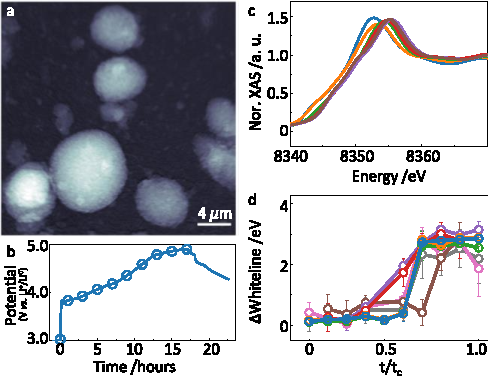
\includegraphics{figures/nca_txm.pdf}
  \caption{Operando \gls{txm} of \nca{} during first charge. (a) Mean
    optical depth frame of \nca{} particles. (b) Applied potential to
    operando cell during galvanostatic charging at
    \SI{0.05}{\ampere\per\ampere\per\hour} (C/20). (c) Normalized spectra
    from \emph{ex-situ} ensemble-average \gls{xas}. (d)
    State-of-charge determined by whiteline position relative to
    overall state of charge in (c) for individual particles of
    \nca{}. Error bars represent one standard deviation over pixels
    within the given particle.}
  \label{fig:txm-nca}
\end{figure}

\begin{figure}[!h]
  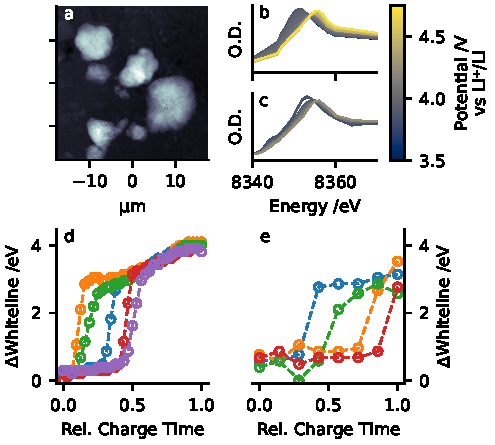
\includegraphics{figures/nmc_txm.pdf}
  \caption{Operando \gls{txm} \gls{xas} of \nmc[333]{} and \nmc[532]{}
    during first charge. (a) Mean optical depth frame of \nmc[333]{}
    particles. (b,c) Median optical depth spectra of active material
    during (b) second charge of \nmc[333]{} and (c) first charge of
    \nmc[532]{}. (d,e) Changes in median whiteline energies during
    first charge relative to start of charging for individual
    particles of (d) \nmc[333]{} (e) \nmc[532]{}.}
  \label{fig:txm-nmc}
\end{figure}

\newpage
\begin{figure}[!h]
    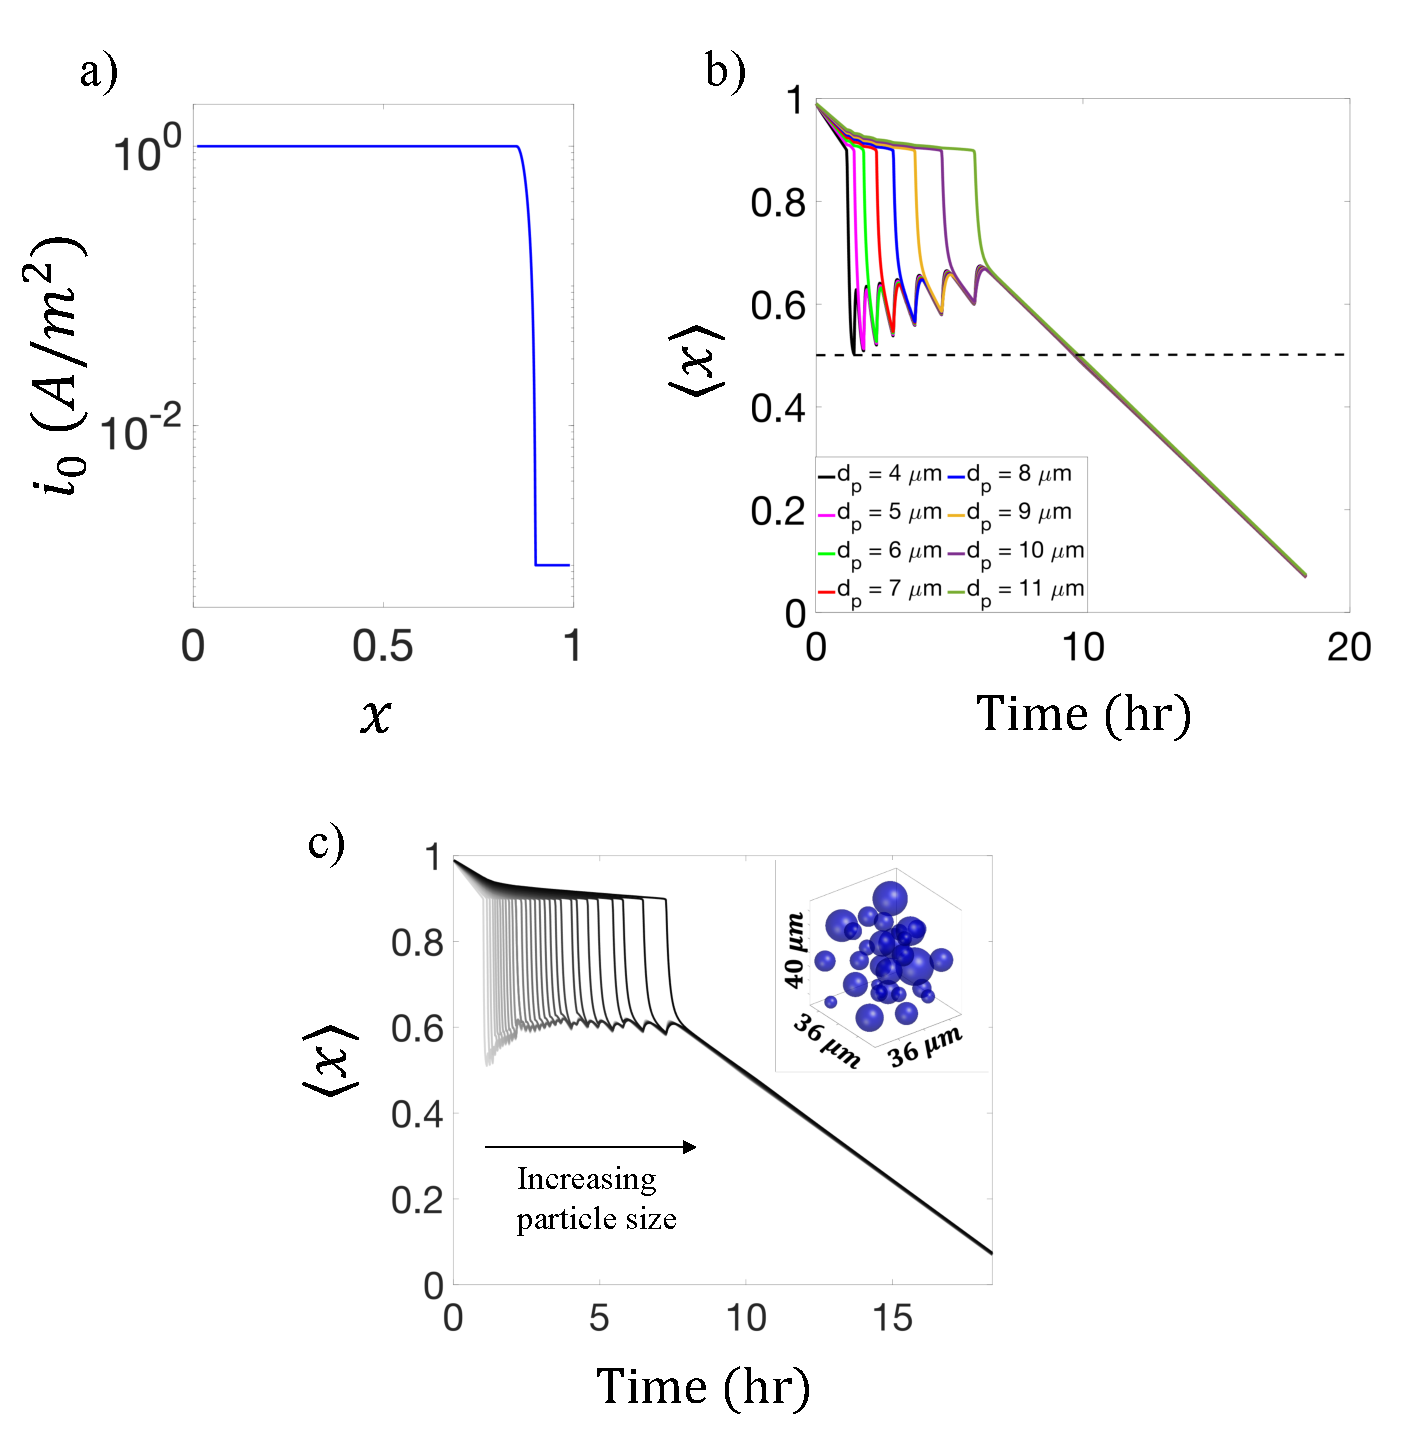
\includegraphics[scale =0.7]{figures/modeling_figure_1.pdf}
    \caption{\todo[inline]{KT: Please match the fonts with the style
        used in experimental plots.  The fonts are too different in
        size, so if they are shrunk so that the axis labels are small
        enough, other fonts will be too small to read.  Please use the
        same font as well.} Simulation results for C/20 galvanostatic
      charging. (a) The model form of \gls{ecd} vs.\ \gls{xLi} used
      for the simulation. The evolution of the volume-averaged
      \gls{xLi} in individual particle, $\langle x \rangle$, for (b)
      the 8-particle system and (c) 30-particle system.}
    \label{fig:model-1}
\end{figure}

\newpage
\begin{figure}[!h]
    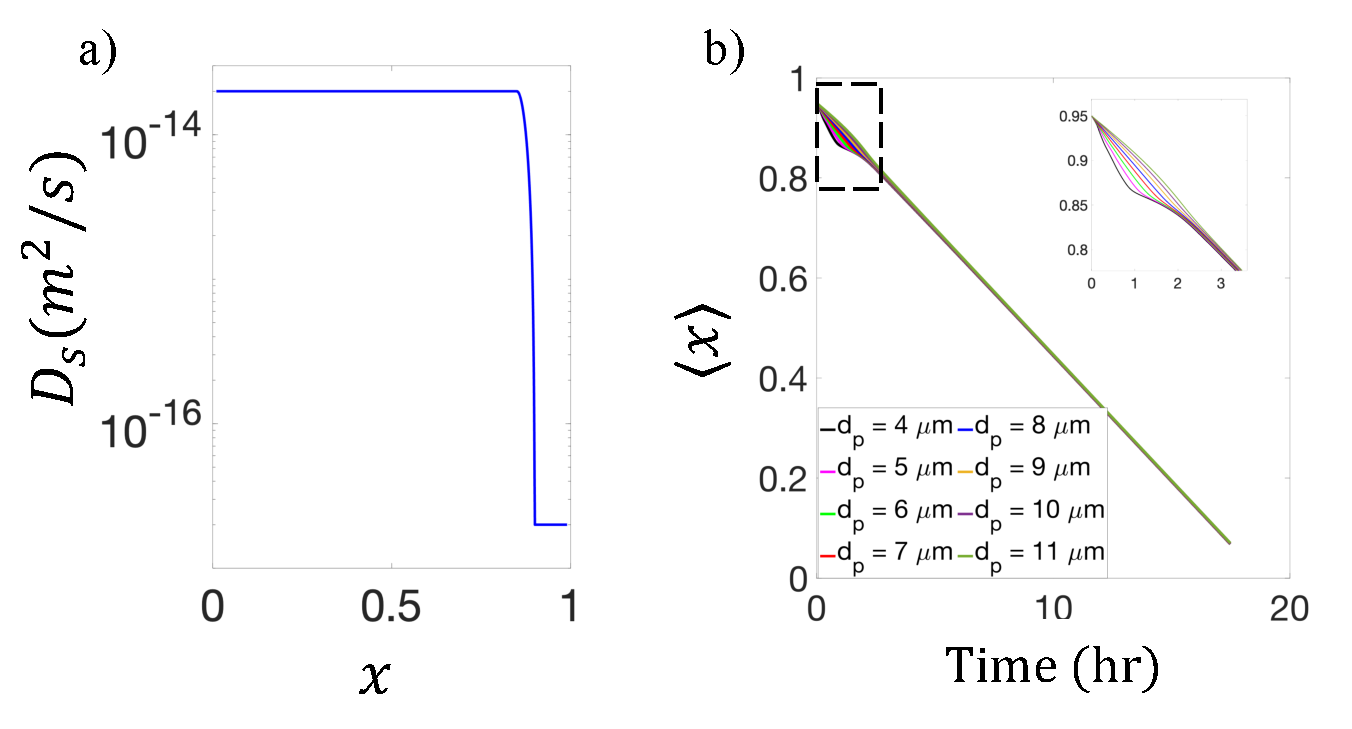
\includegraphics[scale =0.7]{figures/modeling_figure_2_with_Ds_1000_cs_0.95.pdf}
    \caption{\todo[inline]{KT: same} Simulation results for C/20
      galvanostatic charging. (a) The model form of \gls{D_s}
      vs.\ \gls{xLi} used for the simulation. Note that the form is
      the same in terms of the ratio between minimum and maximum
      values and the transition-zone width as that of \gls{ecd} shown
      above. (b) The evolution of the volume-averaged \gls{xLi} in
      individual particle, $\langle x \rangle$, for the 8-particle
      system. The inset shows the zoomed in version of the section
      highlighted using the dashed box.}
    \label{fig:model-2}
\end{figure}


\newpage
\bibliographystyle{plain}
\bibliography{refs,refs-extra}
%% \bibliography{references}

\end{document}
